\documentclass[10pt]{article}
\usepackage[margin=1in]{geometry}
\usepackage[T1]{fontenc}
\usepackage{lmodern}
\usepackage{amsmath,amssymb,amsthm}
\usepackage{booktabs}
\usepackage{graphicx}
\usepackage{xcolor}
\usepackage{listings}
\usepackage{caption}
\usepackage{float}
\usepackage[hidelinks]{hyperref}

\graphicspath{{../figures/}}
\definecolor{codegray}{HTML}{52514E}
\lstset{basicstyle=\ttfamily\small, columns=fullflexible, keepspaces=true, frame=single,
        rulecolor=\color{codegray!40}, xleftmargin=2pt, xrightmargin=2pt, showstringspaces=false}
\newtheorem{proposition}{Proposition}
\newcommand{\R}{\mathbb{R}}
\newcommand{\hL}{h_L^{(\ell)}}
\newcommand{\hS}{h_S^{(s)}}

\title{The $L \to S$ Mapping Function:\\Definition, Estimation, and Properties}
\author{\texttt{weightmap} --- training-free maps between language models\\
\small\url{https://github.com/NISH1001/weightmap}}
\date{November 2026}

\begin{document}
\maketitle

\begin{abstract}
This note gives the exact mapping function used in the \texttt{weightmap} experiments to relate a large
language model $L$ to a small one $S$. The map is affine. It acts on residual-stream states at aligned
tokens, it is estimated in closed form by ridge regression, and nothing is trained. On held-out content
text it explains $R^2 \approx 0.66$ of $S$'s state variance from $L$'s (Qwen2.5-1.5B $\to$ 0.5B), against
$-0.15$ for a shuffled-pairing control. It is effectively linear: random-feature non-linearities add
nothing. It is pruning-like: a subset of $896$ of $L$'s $1536$ coordinates suffices. It holds across model
families and composes almost losslessly along a chain of models. It does \emph{not} transfer capability:
edits derived from $L$ and pushed through the map never improved $S$.
\end{abstract}

\section{Setting and notation}
Let $L$ and $S$ be decoder-only causal language models with $n_L$ and $n_S$ layers and residual widths
$d_L$ and $d_S$. In the main experiment $L$ is Qwen2.5-1.5B-Instruct ($n_L=28$, $d_L=1536$) and $S$ is
Qwen2.5-0.5B-Instruct ($n_S=24$, $d_S=896$). For a text $x$ and token position $t$, write
$h_L^{(\ell)}(x,t)\in\R^{d_L}$ for $L$'s residual-stream state after decoder layer $\ell$, and
$h_S^{(s)}(x,t)\in\R^{d_S}$ likewise for $S$.

\section{Definition}
For a small-model layer $s$ paired with a large-model layer $\ell = \pi(s)$ (Section~\ref{sec:pairing}),
the map is
\begin{equation}
\boxed{\;\hat h_S^{(s)} \;=\; f_s\!\left(\hL\right) \;=\; W_s^{\top}\,\hL + b_s, \qquad
W_s \in \R^{d_L \times d_S},\;\; b_s \in \R^{d_S}.\;}
\label{eq:f}
\end{equation}
It is applied token by token: $\hL$ is evaluated at a token of $L$ and the prediction targets the
\emph{aligned} token of $S$ (Section~\ref{sec:align}). In the main experiment, $\pi(10)=13$ and
$\pi(14)=17$, and $W_s \in \R^{1536\times 896}$.

\section{Estimation}

\subsection{Token alignment}\label{sec:align}
Let $\mathrm{end}_L(i)$ be the character offset at which $L$'s $i$-th token ends, and define
$\mathrm{end}_S(j)$ likewise. Token pairs are
\begin{equation}
\mathcal{P}(x) = \{(i,j) : \mathrm{end}_L(i) = \mathrm{end}_S(j)\},
\end{equation}
excluding padding, zero-width special tokens, and the first real token (an attention sink). At such a pair,
both causal models have read exactly the same text prefix, so their states are comparable. When the two
tokenizers are identical, every position is paired. Up to $k$ pairs per text are sampled at random
($k=32$--$40$).

\subsection{Data matrices}
Stacking the paired states over the fitting texts gives $X\in\R^{N\times d_L}$ (rows $\hL$) and
$Y\in\R^{N\times d_S}$ (rows $\hS$). Rows whose norm in either model exceeds $5\times$ the median are
dropped; these are attention-sink and massive-activation tokens. Let $\mu_X,\mu_Y$ be the column means and
$X_c = X - \mathbf{1}\mu_X^\top$, $Y_c = Y - \mathbf{1}\mu_Y^\top$.

\subsection{Closed-form ridge}
\begin{equation}
W_s = \left(X_c^\top X_c + \lambda I_{d_L}\right)^{-1} X_c^\top Y_c, \qquad
b_s = \mu_Y - W_s^\top \mu_X,
\label{eq:ridge}
\end{equation}
with a scale-free penalty
\begin{equation}
\lambda = \lambda_{\mathrm{rel}} \cdot \overline{\mathrm{Var}}(X)\cdot N, \qquad
\lambda_{\mathrm{rel}} \in \{10^{-4}, 10^{-3}, 10^{-2}, 10^{-1}\},
\end{equation}
where $\overline{\mathrm{Var}}(X)$ is the mean per-column variance. $\lambda_{\mathrm{rel}}$ is chosen by
held-out $R^2$, and the final map is refit on all training rows. This is the only fitted object; neither
$L$ nor $S$ is modified or trained.

\subsection{Evaluation}
Quality is the variance-weighted held-out coefficient of determination
\begin{equation}
R^2 = 1 - \frac{\sum_{n\in\mathcal{T}} \lVert y_n - f(x_n)\rVert^2}{\sum_{n\in\mathcal{T}} \lVert y_n - \bar y\rVert^2},
\end{equation}
where the test set $\mathcal{T}$ consists of \emph{whole held-out texts}: every token of a text sits on one
side of the split. Two controls accompany every map:
\begin{itemize}
  \item \textbf{shuffled pairing:} fit on training rows with the $X\leftrightarrow Y$ pairing permuted,
        evaluate on true pairs;
  \item \textbf{self-reference:} predict $\hS$ from $S$'s own previous layer $h_S^{(s-1)}$, giving a ceiling
        for ``as related as adjacent layers of one model''.
\end{itemize}

\subsection{Layer pairing}\label{sec:pairing}
\begin{equation}
\pi(s) = \arg\max_{\ell'} \; \mathrm{CKA}\!\left(H_S^{(s)}, H_L^{(\ell')}\right), \qquad
\mathrm{CKA}(A,B) = \frac{\lVert A_c^\top B_c\rVert_F^2}{\lVert A_c^\top A_c\rVert_F\,\lVert B_c^\top B_c\rVert_F}.
\end{equation}
The resulting correspondence is almost monotone (Figure~\ref{fig:cka}). Pairing instead by held-out
$R^2$ picks different layers across model families but gives the same map quality (within $0.01$), because
neighbouring large-model layers predict a small-model layer about equally well.

\begin{figure}[t]
\centering
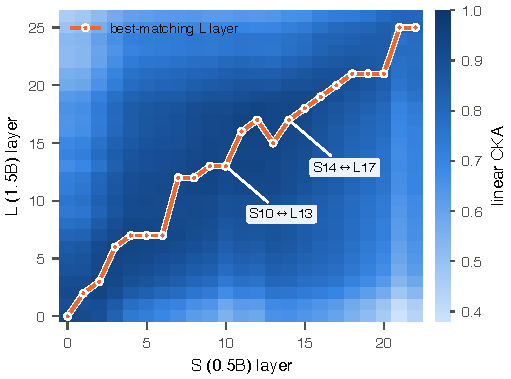
\includegraphics[width=0.48\linewidth]{fig2_cka_layers.pdf}
\caption{Linear CKA between every $S$ layer (Qwen2.5-0.5B) and every $L$ layer (Qwen2.5-1.5B); the line is
$\pi(s)$.}
\label{fig:cka}
\end{figure}

\section{Quality}
\begin{table}[H]
\centering
\caption{Held-out $R^2$ of $f$ (Qwen2.5-0.5B $\leftarrow$ 1.5B; text-level holdout; content text).}
\label{tab:quality}
\begin{tabular}{lcccc}
\toprule
Pair & $R^2_{L\to S}$ & $R^2_{S\to L}$ & shuffled & $S^{(s-1)}\!\to S^{(s)}$ \\
\midrule
$S_{10}\leftarrow L_{13}$ & 0.664 & 0.621 & $-0.154$ & 0.914 \\
$S_{14}\leftarrow L_{17}$ & 0.673 & 0.632 & $-0.156$ & 0.862 \\
\bottomrule
\end{tabular}
\end{table}

\paragraph{Template inflation.} Fitting and scoring on chat-formatted text (system prompt + template +
answer) gives $R^2 = 0.85$ ($0.83$ with text-level holdout). The system prompt and template tokens repeat in
every text and are trivially predictable. The content-level figure in Table~\ref{tab:quality} is the
meaningful one.

\paragraph{Across families.} With SmolLM2-360M as $S$ (a different tokenizer and training corpus) and
Qwen2.5-1.5B as $L$, $R^2_{L\to S} = 0.66$--$0.68$. Across five small models from four families,
$R^2_{S\to L}$ rises with the small model's capability (Spearman $\rho = 0.9$ against bits per byte;
Figure~\ref{fig:atlas}).

\begin{figure}[t]
\centering
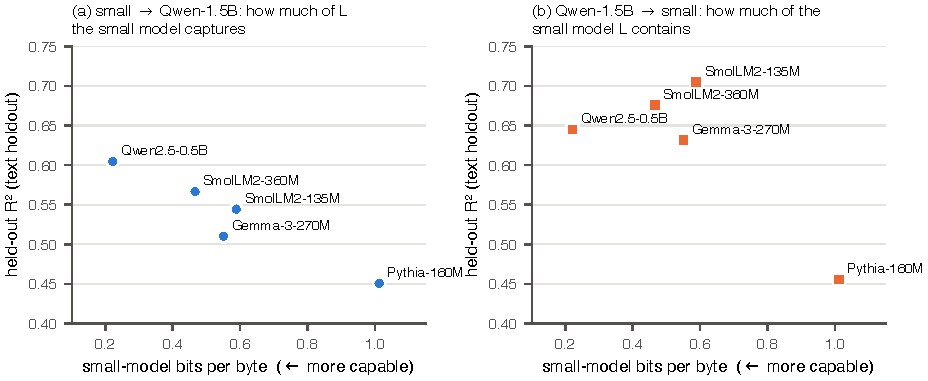
\includegraphics[width=\linewidth]{fig6_atlas.pdf}
\caption{Atlas: five small models mapped onto Qwen2.5-1.5B. (a) $R^2_{S\to L}$ tracks capability;
(b) $R^2_{L\to S}$ measures containment.}
\label{fig:atlas}
\end{figure}

\section{Derived operators}
\begin{table}[H]
\centering
\caption{Operators built from $f_s$ and used in the experiments.}
\begin{tabular}{ll}
\toprule
Operation & Formula \\
\midrule
translate a state & $\hat h_S = W_s^\top h_L + b_s$ \\
transport a direction & $d_S = W_s^\top d_L$ \quad (linear part only) \\
contrast direction & $d_L = \overline{h_L}(\text{L's correct answers}) - \overline{h_L}(\text{S's wrong answers})$ \\
steer $S$ & $h_S \leftarrow h_S + c\,\lVert d_S^{\mathrm{own}}\rVert\, d_S/\lVert d_S\rVert$, \quad $c\in\{1,2,4\}$ \\
transplant & $h_S \leftarrow (1-\beta)\,h_S + \beta\,(W_s^\top h_L + b_s)$ on prompt tokens, \quad $\beta\in\{0.5,1\}$ \\
reverse map & $\hat h_L = W_s'^\top h_S + b_s'$, \quad $W_s'\in\R^{d_S\times d_L}$ (Eq.~\ref{eq:ridge} with $X\leftrightarrow Y$) \\
\bottomrule
\end{tabular}
\end{table}

\begin{proposition}[Folding a steering vector into the weights]
Let layer $s$ of $S$ compute $h \mapsto h + \mathrm{Attn}(h) + \mathrm{MLP}(h')$ with
$\mathrm{MLP}(u) = W_{\mathrm{down}}\,\phi(u)$. Replacing $W_{\mathrm{down}}\phi(u)$ by
$W_{\mathrm{down}}\phi(u) + v$, i.e.\ giving \texttt{down\_proj} the bias $v$, is exactly equivalent to
adding $v$ to the residual stream after layer $s$ at every position.
\end{proposition}
\begin{proof}
The layer output is a sum, and $v$ enters that sum once per position in both cases.
\end{proof}
\noindent This edits $d_S = 896$ parameters ($0.00018\%$ of $S$). In float32 the folded model and the
hook-based steering agree to $1.4\times10^{-4}$ in the logits, at a logit scale of about $32$.

\section{Structure of $f$}

\paragraph{Linear.} Augmenting $X$ with $4096$ random Fourier features $\sqrt{2/D}\cos(\Omega^\top x + \phi)$
(bandwidths $0.5$, $1$, $2\times$ the median distance), which is still a closed-form fit, does not improve the
map: $0.638 \to 0.605$ and $0.650 \to 0.620$. Within this data regime $f$ is effectively linear.

\paragraph{Pruning-like.} Restrict $f$ to a subset $I$ of $L$'s coordinates:
\begin{equation}
\hat h_S = W_{I}^{\top}\, h_L[I] + b, \qquad I = \operatorname{top}_{k}\, \lVert (W_s)_{i,:}\rVert_2 .
\end{equation}
\begin{table}[H]
\centering
\caption{$R^2_{L\to S}$ with $k$ of $L$'s $1536$ coordinates ($S_{10}\leftarrow L_{13}$ / $S_{14}\leftarrow L_{17}$).
The full map already has rank $\le 896$.}
\begin{tabular}{lcccc}
\toprule
$k$ & axis selection & PCA top-$k$ & random axes & all 1536 \\
\midrule
896 & \textbf{0.641 / 0.650} & 0.626 / 0.641 & 0.577 / 0.588 & 0.638 / 0.650 \\
448 & \textbf{0.620 / 0.625} & 0.584 / 0.607 & -- & \\
224 & \textbf{0.557 / 0.563} & 0.530 / 0.560 & -- & \\
\bottomrule
\end{tabular}
\end{table}
Selecting $896$ of $L$'s own coordinates matches the best linear map, so $S$ behaves like a linear readout
of a \emph{subset} of $L$'s neurons. (The PCA baseline is unsupervised, so the clean claim is that
selection reaches the optimum, not that axes beat rotations.)

\paragraph{Weight level.} The same estimator applied to the word-embedding tables (one row per token)
gives $R^2 = 0.31$ (Qwen $\to$ Qwen) and $0.42$ (Qwen $\to$ SmolLM2, $39{,}237$ shared token strings): a
weight-space map exists but is about half as strong as the representation-space map.

\section{Composition}
For a chain of models $M_0 \to M_1 \to \dots \to M_K$ with step maps $f_k(h) = W_k^\top h + b_k$,
\begin{equation}
f_{0\to K} \;\approx\; f_K \circ \dots \circ f_1, \qquad
W_{0\to K} = W_1 W_2 \cdots W_K, \quad
b_{0\to k} = W_k^\top b_{0\to k-1} + b_k \;\;(b_{0\to 1} = b_1).
\end{equation}
\begin{table}[H]
\centering
\caption{Direct vs composed maps along Qwen2.5-1.5B $\to$ Qwen2.5-0.5B $\to$ SmolLM2-360M $\to$ SmolLM2-135M
(layer $\approx 45\%$ depth; text-level holdout).}
\label{tab:comp}
\begin{tabular}{lcccc}
\toprule
End-to-end & direct & composed & composed/direct & $\prod$ step $R^2$ \\
\midrule
1.5B $\to$ 360M & 0.653 & 0.637 & 0.975 & 0.42 \\
0.5B $\to$ 135M & 0.657 & 0.649 & 0.988 & 0.47 \\
1.5B $\to$ 135M & 0.659 & 0.629 & 0.955 & 0.30 \\
\bottomrule
\end{tabular}
\end{table}
Composition keeps $95$--$99\%$ of the direct map, and errors do not compound: the composed $R^2$ is far
above the product of step $R^2$ values. Each step discards mostly what the next, smaller model does not
represent anyway (Figure~\ref{fig:rec}).

\begin{figure}[t]
\centering
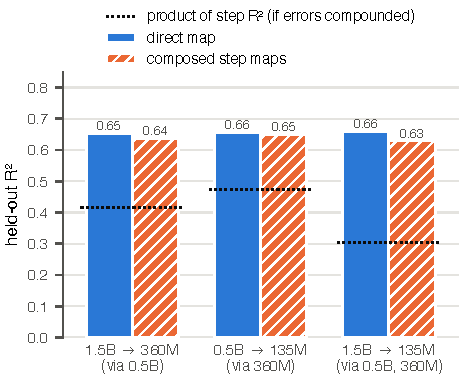
\includegraphics[width=0.5\linewidth]{fig7_recursion.pdf}
\caption{Composed step maps vs direct maps; the dotted line is the product of step $R^2$ values.}
\label{fig:rec}
\end{figure}

\section{What $f$ does not do}
Transporting $L$'s correct-vs-wrong direction into $S$ and steering with it, or transplanting $L$'s mapped
prompt states, never improved $S$ on held-out problems: MATH-500 $\Delta = -0.9$ points, 95\% CI $[-7.3,+5.5]$;
NQ-Open $\Delta = -3.7$ points, CI $[-6.0,-1.3]$. It fixed $0/9$ problems that $S$ never solves. The
transported direction is nearly $S$'s own ($\cos = 0.85$). Because $f$ is a lossy, many-to-one projection,
it discards exactly the component of $L$'s representation that $S$ cannot express. The map explains why
$S$ resembles $L$, not how to make $S$ as capable as $L$.

\section{Reproduction}
\begin{lstlisting}[language=Python]
from weightmap import WeightMap

wm = WeightMap(large="Qwen/Qwen2.5-1.5B-Instruct",
               small="Qwen/Qwen2.5-0.5B-Instruct").fit(texts, layers=[10])
m = wm.maps[10]                       # pi(10) = m.large_layer = 13
W, b = m.large_to_small.W, m.large_to_small.b   # W: [1536, 896], b: [896]
h_small_hat = h_large @ W + b         # identical to wm.to_small(h_large, 10)
print(wm.report())                    # R^2 both ways, shuffled control, self-reference
\end{lstlisting}
The exact entries of $W_s$ depend on the fitting texts; refitting on the same texts reproduces them.
Full experimental details, every table, and threats to validity are in \texttt{docs/EXPERIMENTS.md}.

\end{document}
